%
% File acl2014.tex
%
% Contact: koller@ling.uni-potsdam.de, yusuke@nii.ac.jp
%%
%% Based on the style files for ACL-2013, which were, in turn,
%% Based on the style files for ACL-2012, which were, in turn,
%% based on the style files for ACL-2011, which were, in turn,
%% based on the style files for ACL-2010, which were, in turn,
%% based on the style files for ACL-IJCNLP-2009, which were, in turn,
%% based on the style files for EACL-2009 and IJCNLP-2008...

%% Based on the style files for EACL 2006 by
%%e.agirre@ehu.es or Sergi.Balari@uab.es
%% and that of ACL 08 by Joakim Nivre and Noah Smith

\documentclass[11pt]{article}
\usepackage{style/acl2014}
\usepackage{times}
\usepackage{url}
\usepackage{latexsym}

%%%%%%%%%%%%%%%%%%%%%%%%%%%%%%%%%%%%%%%%%%%%%%%%%%

\usepackage{booktabs}
\usepackage{algorithm}
\usepackage[noend]{algorithmic}
%\usepackage[caption=false]{subfig}
\usepackage[table]{xcolor}
\usepackage{subfigure}

\usepackage{style/mfirstuc}
\newcommand{\etal}[2]{\makefirstuc{#1}~et~al.~\cite{#1-#2}}
\newcommand{\cd}[1]{\bar{\bm{Q}}_{#1, \cdot}  }
\newcommand{\citet}[1]{\newcite{#1}}

\newif\ifcomment\commentfalse
% Preamble file contains handy macros and most packages you might want to use.
% At the start are packages that conflict with various styles.  Don't add them
% in!  Just put it in your main TeX file instead.

% Do not put either of these (subfigure or subfloat) into the preamble
% - they clash.  Use them in the final LaTeX document
% \usepackage{subfigure}
% \suepackage{subfloat}

% Do not use times in the preamble!  It just causes problems with some
% publication chairs (e.g., ICML 2013).  If you want it, put it in your own
% document.
% \usepackage{times}


% Breaks ACM-SIG style
% \usepackage{titlesec}
% \usepackage{amsthm}
% \usepackage{nomencl}

% comment out the following line, as it conflicts with aistats2012.sty
%\usepackage{caption}

% This is required by NSF.  Do not remove; if it conflicts with
% another package, fix that problem without removing this from
% Preamble.
% Unless for AAAI ... this needs a new bibfile that plays well with hyperref.
%\usepackage[a-1b]{pdfx}

% Below should be safe
\usepackage{framed}
\usepackage{mdwlist}
\usepackage{latexsym}
\usepackage{colortbl}
\usepackage{xcolor}
\usepackage{nicefrac}
\usepackage{booktabs}
\usepackage{amsfonts}
\usepackage[T1]{fontenc}
\usepackage{bold-extra}
\usepackage{amsmath}
\usepackage{amssymb}
\usepackage{bm}
\usepackage{graphicx}
\usepackage{mathtools}
\usepackage{microtype}
\usepackage{multirow}
\usepackage{multicol}
% Don't use hyperref or url, as it can screw up AAAI / ICML formatting
%\usepackage{url}
\usepackage{latexsym,comment}
\usepackage[normalem]{ulem}

\newcommand{\breakalign}{\right. \nonumber \\ & \left. \hspace{2cm}}



\newcommand{\feat}[1]{{\small \texttt{#1}}}
\newcommand{\act}[1]{{\small \texttt{#1}}}
\newcommand{\ngram}[0]{$n$-gram}
\newcommand{\topic}[1]{\underline{#1}}
\newcommand{\gem}[1]{\mbox{\textsc{gem}}}
\newcommand{\abr}[1]{\textsc{#1}}
\newcommand{\camelabr}[2]{{\small #1}{\textsc{#2}}}
\newcommand{\abrcamel}[2]{{\textsc #1}{\small{#2}}}
\newcommand{\grammar}[1]{{\color{red} #1}}
\newcommand{\explain}[2]{\underbrace{#2}_{\mbox{\footnotesize{#1}}}}
\newcommand{\dir}[1]{\mbox{Dir}(#1)}
\newcommand{\bet}[1]{\mbox{Beta}(#1)}
\newcommand{\py}[1]{\mbox{\textsc{py}}(#1)}
\newcommand{\td}[2]{\mbox{\textsc{TreeDist}}_{#1} \left( #2 \right)}
\newcommand{\yield}[1]{\mbox{\textsc{Yield}} \left( #1 \right)}
\newcommand{\mult}[1]{\mbox{Mult}( #1)}
\newcommand{\wn}{\textsc{WordNet}}
\newcommand{\twentynews}{\textsc{20news}}
\newcommand{\g}{\, | \,}
\newcommand{\Gam}[1]{\Gamma \left( \textstyle #1 \right)}
\newcommand{\LG}[1]{\log \Gamma \left( \textstyle #1 \right)}
\newcommand{\Pois}[1]{\mbox{Poisson}(#1)}
\newcommand{\pcfg}[3]{#1_{#2 \rightarrow #3}}
\newcommand{\grule}[2]{#1 \rightarrow #2}
\newcommand{\kl}[2]{D_{\mbox{\textsc{KL}}} \left( #1 \,||\, #2 \right)}

\newcommand{\digambig}[1]{\Psi \left( #1 \right) }
\newcommand{\digam}[1]{\Psi \left( \textstyle #1 \right) }
\newcommand{\ddigam}[1]{\Psi' \left( \textstyle #1 \right) }


\renewenvironment{quote}
               {\list{}{\rightmargin\leftmargin}%
                \item\relax\small\ignorespaces}
               {\unskip\unskip\endlist}

\DeclareMathOperator*{\argmax}{arg\,max}
\DeclareMathOperator*{\argmin}{arg\,min}
\newcommand{\bmat}[1]{\text{\textbf{#1}}}
\newcommand{\bvec}[1]{\boldsymbol{#1}}

%\newcommand{\email}[1]{ {\small \href{mailto://#1}{\texttt{#1} }  }}
\newcommand{\emaillink}[1]{ {\small \href{mailto://#1}{\texttt{#1}}}}
\newcommand{\smallemaillink}[2]{ {\small \href{mailto://#2}{\texttt{#1}}}}

% JBG: Consider renaming from \ch to \zh because of conflict when adding Cyrillic
\newcommand{\ch}[1]{\begin{CJK*}{UTF8}{gbsn}#1\end{CJK*}}

\newcommand{\e}[2]{\mathbb{E}_{#1}\left[ #2 \right] }
\newcommand{\h}[2]{\mathbb{H}_{#1}\left[ #2 \right] }
\newcommand{\ind}[1]{\mathds{1}\left[ #1 \right] }
\newcommand{\ex}[1]{\mbox{exp}\left\{ #1\right\} }
\newcommand{\D}[2]{\frac{\partial #1}{\partial #2}}
\newcommand{\elbo}{\mathcal{L}}

\newcommand{\hidetext}[1]{}
\newcommand{\ignore}[1]{}

\newcommand{\todo}[1]{\textcolor{red}{{\bf TODO: #1}}}

\ifcomment
\newcommand{\pinaforecomment}[3]{\colorbox{#1}{\parbox{.8\linewidth}{#2: #3}}}
\else
\newcommand{\pinaforecomment}[3]{}
\fi

\newcommand{\jbgcomment}[1]{\pinaforecomment{red}{JBG}{#1}}
\newcommand{\mjpcomment}[1]{\pinaforecomment{blue}{MJP}{#1}}
\newcommand{\czcomment}[1]{\pinaforecomment{orange}{chen}{#1}}
\newcommand{\ffcomment}[1]{\pinaforecomment{red}{FF}{#1}}
\newcommand{\fpcomment}[1]{\pinaforecomment{green}{FP}{#1}}
\newcommand{\yhcomment}[1]{\pinaforecomment{green}{YH}{#1}}
\newcommand{\hhecomment}[1]{\pinaforecomment{blue}{HH}{#1}}
\newcommand{\tncomment}[1]{\pinaforecomment{blue}{TN}{#1}}
\newcommand{\mnicomment}[1]{\pinaforecomment{green}{Mohit}{#1}}
\newcommand{\prcomment}[1]{\pinaforecomment{lightblue}{Pedro}{#1}}
\newcommand{\fscomment}[1]{\pinaforecomment{orange}{Shi}{#1}}
\newcommand{\vmcomment}[1]{\pinaforecomment{yellow}{Varun}{#1}}
\newcommand{\rscomment}[1]{\pinaforecomment{yellow}{Richard}{#1}}
\newcommand{\jszcomment}[1]{\pinaforecomment{green}{JSG}{#1}}
\newcommand{\ascomment}[1]{\pinaforecomment{blue}{AS}{#1}}
\newcommand{\vecomment}[1]{\pinaforecomment{blue}{VE}{#1}}
\newcommand{\halcomment}[1]{\pinaforecomment{magenta!20}{Hal}{#1}}
\newcommand{\kgcomment}[1]{\pinaforecomment{blue}{Kim}{#1}}
\newcommand{\vancomment}[1]{\pinaforecomment{green}{VAN}{#1}}
\newcommand{\thangcomment}[1]{\pinaforecomment{green}{Thang}{#1}}
\newcommand{\alvincomment}[1]{\pinaforecomment{cyan}{Alvin}{#1}}
\newcommand{\reviewercomment}[1]{\pinaforecomment{blue}{Reviewer}{#1}}
\newcommand{\brscomment}[1]{\pinaforecomment{blue}{BRS}{#1}}
\newcommand{\psrcomment}[1]{\pinaforecomment{yellow}{PSR}{#1}}
\newcommand{\zkcomment}[1]{\pinaforecomment{cyan}{ZK}{#1}}
\newcommand{\swcomment}[1]{\pinaforecomment{yellow}{SW}{#1}}
\newcommand{\shaycomment}[1]{\pinaforecomment{yellow}{SBC}{#1}}
\newcommand{\jlundcomment}[1]{\pinaforecomment{cyan}{J}{#1}}
\newcommand{\kdscomment}[1]{\pinaforecomment{ceil}{KDS}{#1}}
\newcommand{\lkfcomment}[1]{\pinaforecomment{yellow}{LF}{#1}}
\newcommand{\yfcomment}[1]{\pinaforecomment{brown}{YF}{#1}}
\newcommand{\ewcomment}[1]{\pinaforecomment{lightblue}{Eric}{#1}}
\newcommand{\pgcomment}[1]{\pinaforecomment{cyan}{Pranav}{#1}}
\newcommand{\bencomment}[1]{\pinaforecomment{lightblue}{Ben}{#1}}

\newcommand{\smalltt}[1]{ {\tt \small #1 }}
\newcommand{\smallurl}[1]{ \begin{tiny}\url{#1}\end{tiny}}
%\newcommand{\smallurl}[1]{ \begin{tiny} HIDDEN \end{tiny}}
\newenvironment{compactenum}{ \begin{enumerate*} \small }{ \end{enumerate*} }

\definecolor{lightblue}{HTML}{3cc7ea}
\definecolor{CUgold}{HTML}{CFB87C}
\definecolor{grey}{rgb}{0.95,0.95,0.95}
\definecolor{ceil}{rgb}{0.57, 0.63, 0.81}
\definecolor{UMDred}{HTML}{ed1c24}
\definecolor{UMDyellow}{HTML}{ffc20e}

% Datasets / Models

\newcommand{\qb}[0]{Quizbowl}
\newcommand{\qa}[0]{\abr{qa}}
\newcommand{\triviaqa}{\camelabr{Trivia}{qa}}
\newcommand{\searchqa}{\camelabr{Search}{qa}}
\newcommand{\qblink}{\abrcamel{qb}{Link}}
\newcommand{\qanta}{\textsc{qanta}}
\newcommand{\muse}{\textsc{muse}}
\newcommand{\squad}{\textsc{sq}{\small u}\textsc{ad}}
\newcommand{\fever}{\abr{fever}}
\newcommand{\quac}{\textsc{q}{\small u}\textsc{ac}}
\newcommand{\elmo}{\textsc{elm}{\small o}}
\newcommand{\fone}{$F_1$}
\newcommand{\jeopardy}{\textit{Jeopardy!}}

\newcommand{\red}[1]{{\color{red}{\bf #1}}}
\newcommand{\blue}[1]{{\color{blue}{\bf #1}}}
\newcommand{\green}[1]{{\color{green}{\bf #1}}}
\newcommand{\purple}[1]{{\color{purple}{\bf #1}}}
%%%%%%%%%%%%%%%%%%%%%%%%%%%%%%%%%%%%%%%%%%%%%%%%%%

\title{Anchors Regularized: Adding Robustness and Extensibility \\
to Scalable Topic-Modeling Algorithms}

\author{Thang Nguyen  \\
  iSchool and \abr{umiacs}, \\
  University of Maryland \\
  and National Library of Medicine, \\
  National Institutes of Health \\
  \email{daithang@umiacs.umd.edu} \\\And
  Yuening Hu \\
  Computer Science \\
  University of Maryland \\
  \email{ynhu@cs.umd.edu} \\ \And
  Jordan Boyd-Graber \\
  iSchool and \abr{umiacs} \\
  University of Maryland \\
  \email{jbg@umiacs.umd.edu} \\
}

\date{}



\begin{document}

%\maketitle

% TODO
% 1.  Explain different corpora for TI
% 2.  Hyperparameter selection for HL
% 3.  Discussion of HL equivalence, VB and Gibbs competitive
% 4.  Explain why NIPS has poor WIKITI
% 5.  Remove informed prior equation
% 6.  Rewrite final discussion

%\jbgcomment{Took a stab at improving the abstract, but not sure it's all the way
%there yet.}

\begin{abstract}
  Spectral methods offer scalable alternatives to Markov chain Monte
  Carlo and expectation maximization.  However, these new methods lack
  the rich priors associated with probabilistic models.  We examine
  Arora et al.'s anchor words algorithm for topic modeling and develop
  new, regularized algorithms that not only mathematically resemble
  Gaussian and Dirichlet priors but also improve the interpretability
  of topic models.  Our new regularization approaches make these
  efficient algorithms more flexible; we also show that these methods can
  be combined with informed priors.
\end{abstract}

\section{Introduction}
\label{sec:intro}

Topic models are of practical and theoretical interest.  Practically,
they have been used to understand political
perspective~\cite{paul-10}, improve machine
translation~\cite{Eidelman-12}, reveal literary
trends~\cite{jockers-13}, and understand scientific
discourse~\cite{hall-08}.  Theoretically, their latent variable
formulation has served as a foundation for more robust models of other
linguistic phenomena~\cite{brody-09}.

Modern topic models are formulated as a latent variable model.  Like
hidden Markov models~\cite[\abr{hmm}]{rabiner-89}, each token comes
from one of $K$ unknown distributions.  Unlike a \abr{hmm}, topic
models assume that each document is an \emph{admixture} of these
hidden components called topics.  Posterior inference discovers the
hidden variables that best explain a dataset.  Typical solutions use
\abr{mcmc}~\cite{griffiths-04} or variational \abr{em}~\cite{blei-03},
which can be viewed as local optimization: searching for the latent
variables that maximize the data likelihood.

An exciting vein of new research provides provable polynomial-time
alternatives.  These approaches provide solutions to hidden Markov
models~\cite{anandkumar-12:hmm}, mixture models~\cite{kannan-05}, and
latent variable grammars~\cite{cohen-13b}. The key insight is not to
directly optimize observation likelihood but to instead discover
latent variables that can reconstruct statistics of the assumed
generative model.  Unlike search-based methods, which can be caught in
local minima, these techniques are often guaranteed to find global
optima.

These general techniques can be improved by making reasonable
assumptions about the models.  For example, Arora et
al.~\shortcite{Arora-2012b}'s approach for inference in topic models
assume that each topic has a unique ``anchor'' word (thus, we call
this approach {\bf anchor}).  This approach is fast and effective;
because it only uses word co-occurrence information, it can scale to
much larger datasets than \abr{mcmc} or \abr{em} alternatives.  We
review the {\bf anchor} method in Section~\ref{sec:anchor}.

Despite their advantages, these techniques are not a panacea.  They do
not accommodate the rich priors that modelers have come to expect.
Priors can improve performance~\cite{wallach-09b}, provide domain
adaptation~\cite{daume-07,finkel-09}, and guide models to reflect
users' needs~\cite{hu-13:itm}.  In Section~\ref{sec:prior}, we
regularize the {\bf anchor} method to trade-off the reconstruction
fidelity with the penalty terms that mimic Gaussian and Dirichlet
priors.

Another shortcoming is that these models have not been scrutinized
using standard \abr{nlp} evaluations.  Because these approaches
emerged from the theory community, {\bf anchor}'s evaluations, when
present, typically use training reconstruction.  In
Section~\ref{sec:experiments}, we show that our regularized models can
generalize to previously unseen data---as measured by held-out
likelihood~\cite{blei-03}---and are more
interpretable~\cite{chang-09b,newman-10}.  We also show that our
extension to the {\bf anchor} method enables new applications: for
example, using an informed priors to discover concepts of interest.

Having shown that regularization does improve performance,
in Section~\ref{sec:disc} we explore why.  We discuss the trade-off
of training data reconstruction with sparsity and why regularized
topics are more interpretable.

\section{Anchor Words: Scalable Topic Models}

\label{sec:anchor}
\begin{table}[t!]
\begin{center}

\begin{small}
\rowcolors{1}{}{lightgray}
\begin{tabular}{|l p{6.25cm}| }
\hline
$K$ & number of topics\\
$V$ & vocabulary size\\
$M$ & document frequency: minimum documents an anchor word
candidate must appear in \\
$\bm{Q}$ & word co-occurrence matrix\newline  $Q_{i,j} = p(w_1 = i, w_2 = j) $\\
$\bm{\bar{ Q}}$ & conditional distribution of $Q$\newline  ${\bar Q}_{i,j} = p(w_1 = j \g w_2= i)$ \\
$ \cd{i} $ & row $i$ of ${\bar Q}$ \\
$\bm{A}$ & topic matrix, of size $V \times K$ \newline  $A_{j,k} = p(w=j \g z=k)$ \\
$\bm{C}$ & anchor coefficient of size $K \times V$\newline $C_{j,k} = p(z=k\g
w=j)$ \\
$\mathcal{S}$ & set of anchor word indexes $\{s_1, \dots s_K\}$ \\
$\lambda$ &regularization weight\\
\hline
\end{tabular}
\end{small}
\end{center}
\caption{Notation used.  Matrices are in bold ($\bm{Q}, \bm{C}$), sets are in
  script $\mathcal{S}$}
\label{tab:TableOfNotation}
\end{table}

In this section, we briefly review the {\bf anchor} method and place it in the
context of topic model inference.  Once we have established the {\bf anchor}
objective function, in the next section we regularize the objective function.

\paragraph{Rethinking Data: Word Co-occurrence}

Inference in topic models can be viewed as a black box: given a set of
documents, discover the topics that best explain the data.  The difference
between {\bf anchor} and conventional inference is that while
conventional methods take a collection of documents as input, {\bf anchor}
takes \emph{word co-occurrence} statistics.  Given a vocabulary of size
$V$, we represent this joint distribution as $\bm{Q}_{i,j} = p(w_1 =i, w_2=j)$,
each cell represents the probability of words appearing together in a document.

Like other topic modeling algorithms, the output of the {\bf anchor} method is
the topic word distributions $\bm{A}$ with size $V*K$, where $K$ is the total number
of topics desired, a parameter of the algorithm.  The $k^{th}$ column of $A$
will be the topic distribution over all words for topic $k$, and $\bm{A}_{w,k}$ is
the probability of observing type $w$ given topic $k$.

\paragraph{Anchors: Topic Representatives}

The {\bf anchor} method~\cite{Arora-2012} is based on the separability
assumption~\cite{Donoho-2003}, which assumes that each topic contains at least
one namesake ``anchor word'' that has non-zero probability only in that topic.
Intuitively, this means that each topic has unique, specific word that, when
used, identifies that topic.  For example, while ``run'', ``base'', ``fly'', and
``shortstop'' are associated with a topic about \underline{baseball},
only ``shortstop'' is unambiguous, so it could serve as this topic's anchor word.

Let's assume that we knew what the anchor words were: a set $\mathcal{S}$ that
indexes rows in $\bm{Q}$.  Now consider the {\bf conditional distribution} of word
$i$, the probability of the rest of the vocabulary given an observation of word
$i$; we represent this as $\cd{i}$, as we can construct this by
normalizing the rows of $\bm{Q}$.  For an anchor word $s_a \in
\mathcal{S}$, this will look like a topic; $\cd{\mbox{``shortstop''}}$ will have
high probability for words associated with \underline{baseball}.

The key insight of the {\bf anchor} algorithm is that the conditional
distribution of polysemous non-anchor words can be reconstructed as a
linear combination of the conditional distributions of anchor words.
For example, $\cd{\mbox{``fly''}}$ could be reconstructed by combining
the anchor words ``insecta'', ``boeing'', and ``shortshop''.  We
represent the coefficients of this reconstruction as a matrix
$\bm{C}$, where $C_{i,k} = p(z=k \g w=i)$.  Thus, for any word $i$,
\begin{equation}
  \bar{\bm{Q}}_{i,\cdot} \approx \sum_{s_k \in \mathcal{S}} C_{i,k} \bar{\bm{Q}}_{s_k, \cdot}.
\label{eq:lincomb}
\end{equation}
The coefficient matrix is {\bf not} the usual output of a topic modeling
algorithm.  The usual output is the probability of a word \emph{given a topic}.
The coefficient matrix $C$ is the probability of a topic \emph{given a word}.
We use Bayes rule to recover the topic distribution $p(w=i|z=k) \equiv $
\begin{align}
A_{i,k}  & \propto p(z=k|w=i) p(w=i)  \notag \\
   & = C_{i,k} \sum_{j}
{\bar{Q}_{i,j}}
\label{eq:coef-to-topic}
\end{align}
where $p(w)$ is the normalizer of $\bm{Q}$ to obtain $\cd{w}$.

The geometric argument for finding the anchor words is one of the key
contributions of \citet{Arora-2012} and is beyond the scope of
this paper.  The algorithms in Section~\ref{sec:prior} use the anchor selection
subroutine unchanged.  The difference in our approach is in how we discover the
anchor coefficients $C$.

\paragraph{From Anchors to Topics}

After we have the anchor words, we need to find the coefficients that
best reconstruct the data $\bar{Q}$ (Equation~\ref{eq:lincomb}).
\citet{Arora-2012} chose the $C$ that minimizes the \abr{kl}
divergence between $\bar{Q}_{i,\cdot}$ and the reconstruction based on
the anchor word's conditional word vectors $\sum_{s_k \in \mathcal{S}}
C_{i,k} \cd{s_k}$,
\begin{equation}
\label{eq:anchor}
\begin{small}
\bm{C}_{i,\cdot} = \text{argmin}_{\bm{C}_{i,\cdot}} \kl{\cd{i}}{\sum_{s_k \in S} C_{i,k} \cd{s_k}}.
\end{small}
\end{equation}

The {\bf anchor} method is fast, as it only depends on the size of the
vocabulary once the co-occurrence statistics $\bm Q$ are obtained.  However, it does
not support rich priors for topic models, while \abr{mcmc}~\cite{griffiths-04} and
variational \abr{em}~\cite{blei-03} methods can.  This prevents models from
using priors to guide the models to discover particular themes~\cite{zhai-12},
or to encourage sparsity in the models~\cite{yao-09}.  In the rest of this
paper, we correct this lacuna by adding regularization inspired by Bayesian
priors to the {\bf anchor} algorithm.
\section{Adding Regularization}
\label{sec:prior}

In this section, we add regularizers to the {\bf anchor} objective
(Equation~\ref{eq:anchor}).  In this section, we briefly review regularizers and
then add two regularizers, inspired by Gaussian ($L_2$, Section~\ref{sec:l2})
and Dirichlet priors (Beta, Section~\ref{sec:beta}), to the {\bf anchor}
objective function (Equation~\ref{eq:anchor}).

Regularization terms are ubiquitous.  They typically appear as an
additional term in an optimization problem.  Instead of optimizing a
function just of the data $x$ and parameters $\beta$, $f(x, \beta)$,
one optimizes an objective function that includes a regularizer that
is only a function of parameters: $f(w, \beta) + r(\beta)$.
Regularizers are critical in staid methods like linear
regression~\cite{ng-04}, in workhorse methods such as maximum entropy
modeling~\cite{dudik-04}, and also in emerging fields such as deep
learning~\cite{wager-13}.

In addition to being useful, regularization terms are appealing
theoretically because they often correspond to probabilistic
interpretations of parameters.  For example, if we are seeking the
\abr{mle} of a probabilistic model parameterized by $\beta$, $p(x|
\beta)$, adding a regularization term $r(\beta) = \sum_{i=1}^L
\beta_i^2$ corresponds to adding a Gaussian prior
\begin{equation}
f(\beta_i) = \frac{1}{\sqrt{2\pi\sigma^2}} \ex{-\frac{\beta_i^2}{2\sigma^2}}
\end{equation}
and maximizing log probability of the posterior (ignoring constant
terms)~\cite{Rennie03onl2-norm}.

\subsection{$L_2$ Regularization}
\label{sec:l2}

The simplest form of regularization we can add is $L_2$
regularization.  This is similar to assuming that probability of a
word given a topic comes from a Gaussian distribution.  While the
distribution over topics is typically Dirichlet, Dirichlet
distributions have been replaced by logistic normals in topic modeling
applications~\cite{blei-06} and for probabilistic grammars of
language~\cite{cohen-09}.

Augmenting the {\bf anchor} objective with an $L_2$ penalty yields
\begin{align}
\label{eq:anchorl2}
\bm{C}_{i,\cdot} =& \text{argmin}_{C_{i,\cdot} } \kl{\bar{\bm{Q}}_{i,\cdot}}{\sum_{s_k \in S} C_{i,k} \bar{\bm{Q}}_{s_k,\cdot}} \notag \\
&+\lambda \|\bm{C}_{i,\cdot}\ - \mu_{i, \cdot} \|_2^2,
\end{align}
where regularization weight $\lambda$ balances the importance of a
high-fidelity reconstruction against the regularization, which
encourages the anchor coefficients to be close to the vector
$\mu$. When the mean vector $\mu$ is zero, this encourages the topic
coefficients to be zero.  In Section~\ref{sec:informed}, we use a
non-zero mean $\mu$ to encode an informed prior to encourage topics to
discover specific concepts.


\begin{table}[t]
   \begin{center}
   \begin{tabular}{c c c c c}
   \hline\hline
   Corpus & Train & Dev & Test & Vocab  \\
   \hline
   \abr{nips} & 1231 & 247 & 262 & 12182\\
   \abr{20news} & 11243 & 3760 &3726 &81604\\
   \abr{nyt} & 9255 & 2012 & 1959 & 34940\\
   \hline
   \end{tabular}
   \end{center}
\caption{The number of documents in the train, development, and test folds in
  our three datasets.}
   \label{tab:corpus}
\end{table}


\subsection{Beta Regularization}
\label{sec:beta}

The more common prior for topic models is a Dirichlet
prior~\cite{minka-00}.  However, we cannot apply this directly because the
optimization is done on a row-by-row basis of the anchor coefficient matrix $\bm{C}$,
optimizing $\bm{C}$ for a fixed word $w$ for and all topics.  If we want to model the
probability of a word, it must be the probability of word $w$ in a topic versus all
other words.

Modeling this dichotomy (one versus all others in a topic) is possible.
The constructive definition of the Dirichlet
distribution~\cite{sethuraman-94} states that if one has a
$V$-dimensional multinomial $\theta \sim \dir{\alpha_1 \dots
  \alpha_V}$, then the marginal distribution of $\theta_w$ follows
$\theta_w \sim \bet{\alpha_w, \sum_{i \not = w} \alpha_i}$.  This is
the tool we need to consider the distribution of a single word's
probability.

This requires including the topic matrix as part of the objective function.  The
topic matrix is a linear transformation of the coefficient matrix
(Equation~\ref{eq:coef-to-topic}).  The objective for beta regularization
becomes
\begin{align}
\label{eq:anchorbeta}
\bm{C}_{i,\cdot} = &\text{argmin}_{C_{i,\cdot}} \kl{\cd{i} }{\sum_{s_k \in S} C_{i,k} \cd{s_k}} \notag \\
   &- \lambda \sum_{s_k\in S}\mbox{log (Beta}(A_{i,k};a,b)),
\end{align}
where $\lambda$ again balances reconstruction against the regularization.  To
ensure the tractability of this algorithm, we enforce a convex regularization
function, which requires that $a >1$ and $b>1$.  If
we enforce a uniform prior---$\e{\bet{a,b}}{ A_{i,k}} = \frac{1}{V}$---and
that the \emph{mode} of the distribution is also $\frac{1}{V}$,\footnote{For
  $a,b < 1$, the expected value is still the uniform distribution but the mode
  lies at the boundaries of the simplex.  This corresponds to a sparse Dirichlet
  distribution, which our optimization cannot at present model.} this gives us
the following parametric form for $a$ and $b$:
\begin{equation}
a =\frac{x}{V} +1, \mbox{ and } b=\frac{(V-1)x}{V}+1
\end{equation}
for real $x$ greater than zero.

\subsection{Initialization and Convergence}

Equation~\ref{eq:anchorl2} and Equation~\ref{eq:anchorbeta} are optimized using
\abr{l-bfgs} gradient optimization~\cite{galassi-03}.  We initialize $\bm {C}$
randomly from $\dir{\alpha}$ with $\alpha = \frac{60}{V}$ ~\cite{wallach-09b}.
We update $\bm{C}$ after optimizing all $V$ rows. The newly updated $\bm {C}$
replaces the old topic coefficients.  We track how much the topic coefficients
$\bm{C}$ change between two consecutive iterations $i$ and $i+1$ and represent
it as $\Delta \bm{C} \equiv \|\bm{C}^{i+1}- \bm{C}^i \|_2$.  We stop
optimization when $\Delta \bm{C} \le \delta$.  When $\delta=0.1$, the $L_2$ and
unregularized anchor algorithm converges after a single iteration, while beta
regularization typically converges after fewer than ten iterations (Figure
~\ref{fig:convergence}).

\begin{figure*}[t]
\centering
\subfigure{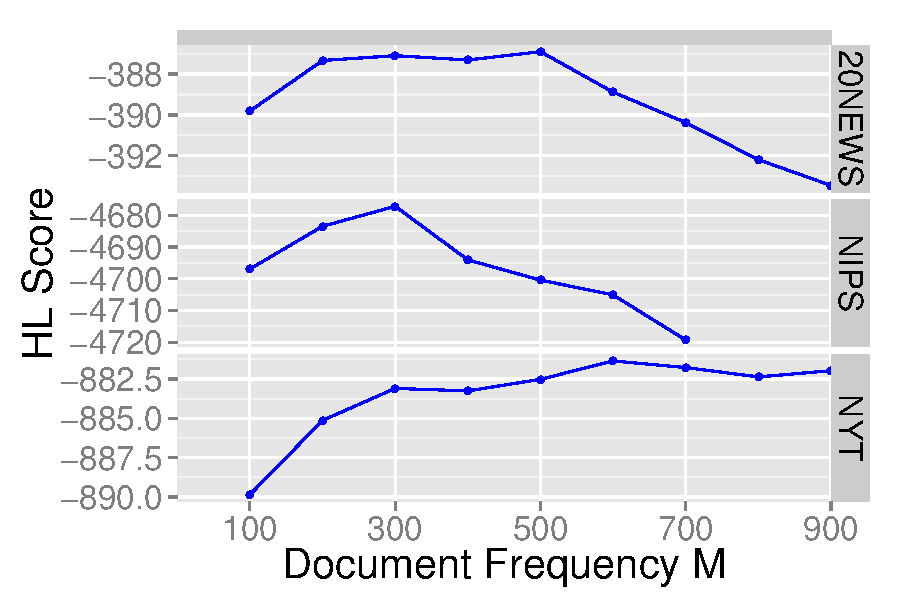
\includegraphics[width=0.48\linewidth]{2014_acl_reganchor/figures/M_HL.pdf}}
\subfigure{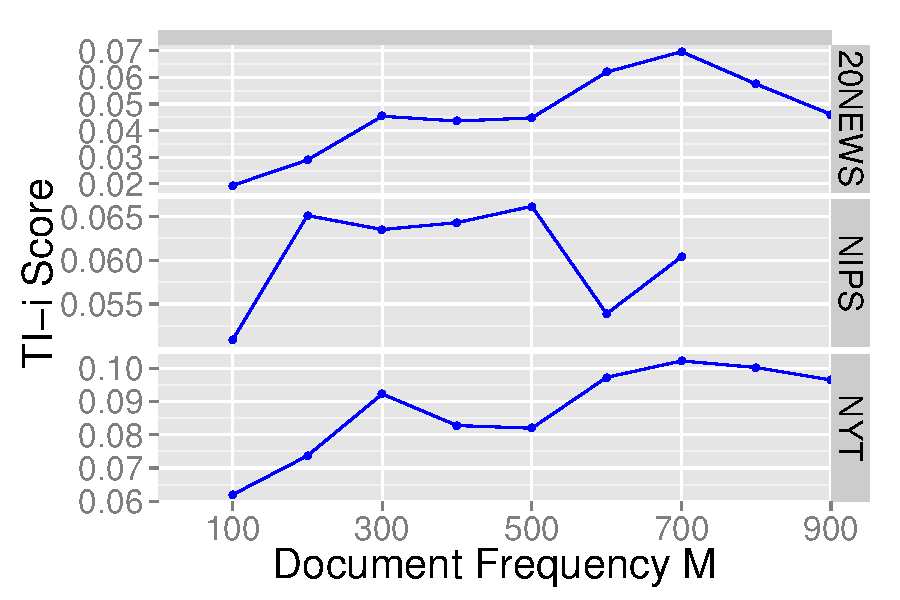
\includegraphics[width=0.48\linewidth]{2014_acl_reganchor/figures/M_TI.pdf}}
\caption{Grid search for document frequency $M$ for our datasets with
  20 topics (other configurations not shown) on development data. The
  performance on both \abr{hl} and \abr{ti} score indicate that the
  unregularized {\bf anchor} algorithm is very sensitive to $M$.  The
  $M$ selected here is applied to subsequent models.}
\label{fig:anchor-select}
\end{figure*}



\section{Regularization Improves Topic Models}
\label{sec:experiments}

In this section, we measure the performance of our proposed
regularized anchor word algorithms.  We will refer to specific
algorithms in bold.  For example, the original anchor algorithm is
{\bf anchor}.  Our $L_2$ regularized variant is {\bf anchor-$L_2$},
and our beta regularized variant is {\bf anchor-beta}.  To provide
conventional baselines, we also compare our methods against topic
models from variational inference \cite[{\bf
  variational}]{blei-03} and \abr{mcmc}~\cite[{\bf
  \abr{mcmc}}]{griffiths-04,mallet}.

We apply these inference strategies on three diverse corpora:
scientific articles from the Neural Information Processing
Society~(\abr{nips}),\footnote{\url{http://cs.nyu.edu/~roweis/data.html}} Internet newsgroups
postings~(\abr{20news}),\footnote{\url{http://qwone.com/~jason/20Newsgroups/}} and New York Times
editorials~\cite[\abr{nyt}]{sandhaus-08}.  Statistics for the datasets
are summarized in Table~\ref{tab:corpus}.  We split each dataset into
a training fold (70\%), development fold (15\%), and a test
fold (15\%): the training data are used to fit models; the development
set are used to select parameters (anchor threshold $M$, document
prior $\alpha$, regularization weight $\lambda$); and final results
are reported on the test fold.

We use two evaluation measures, held-out likelihood \cite[{\bf
  \abr{hl}}]{blei-03} and topic interpretability~\cite[{\bf
  \abr{ti}}]{chang-09b,newman-10}.  Held-out likelihood measures how
well the model can reconstruct held-out documents that the model has
never seen before.  This is the typical evaluation for probabilistic
models.  Topic interpretability is a more recent metric to capture how
useful the topics can be to human users attempting to make sense of a
large datasets.

Held-out likelihood cannot be computed with existing {\bf anchor} algorithms, so
we use the topic distributions learned from {\bf anchor} as input to a reference variational
inference implementation~\cite{blei-03} to compute {\bf \abr{hl}}.
This requires an additional parameter, the Dirichlet prior
$\alpha$ for the per-document distribution over topics.  We select $\alpha$
using grid search on the development set.

To compute {\bf \abr{ti}} and evaluate topic coherence, we use normalized
pairwise mutual information~(\abr{npmi})~\cite{lau-14} over topics' twenty most
probable words.  Topic coherence is computed against the \abr{npmi} of a
reference corpus.  For coherence evaluations, we use both intrinsic and
extrinsic text collections to compute \abr{npmi}.  Intrinsic coherence
(\abr{ti}-i) is computed on training and development data at development time
and on training and test data at test time.
Extrinsic coherence (\abr{ti}-e) is computed from
English Wikipedia articles, with disjoint halves (1.1 million pages each) for distinct
development and testing \abr{ti}-e evaluation.


\begin{figure*}[t!]
\centering
\subfigure{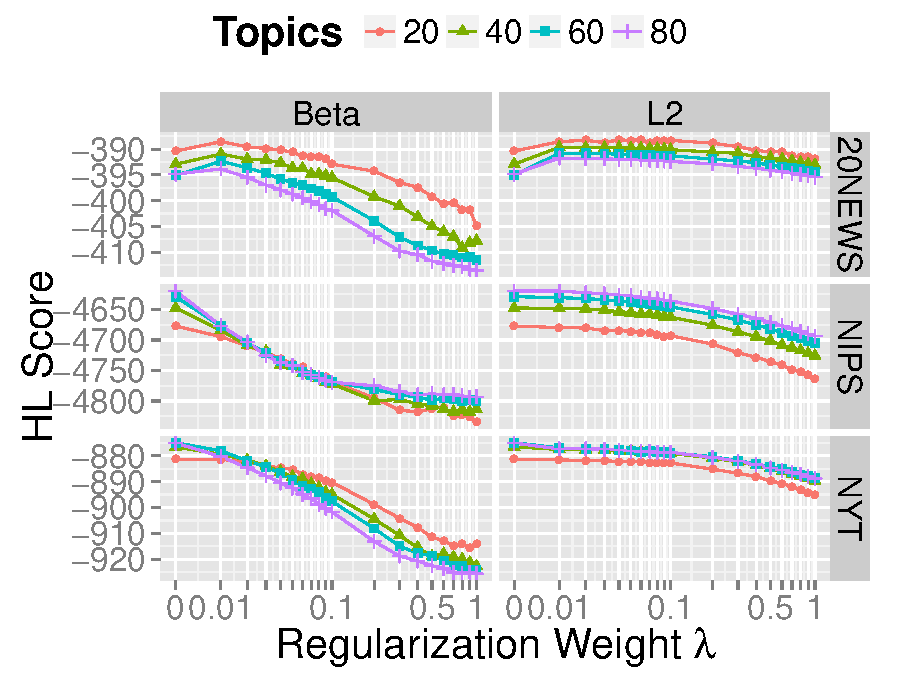
\includegraphics[width=0.48\linewidth]{2014_acl_reganchor/figures/HL_HL.pdf}}
\subfigure{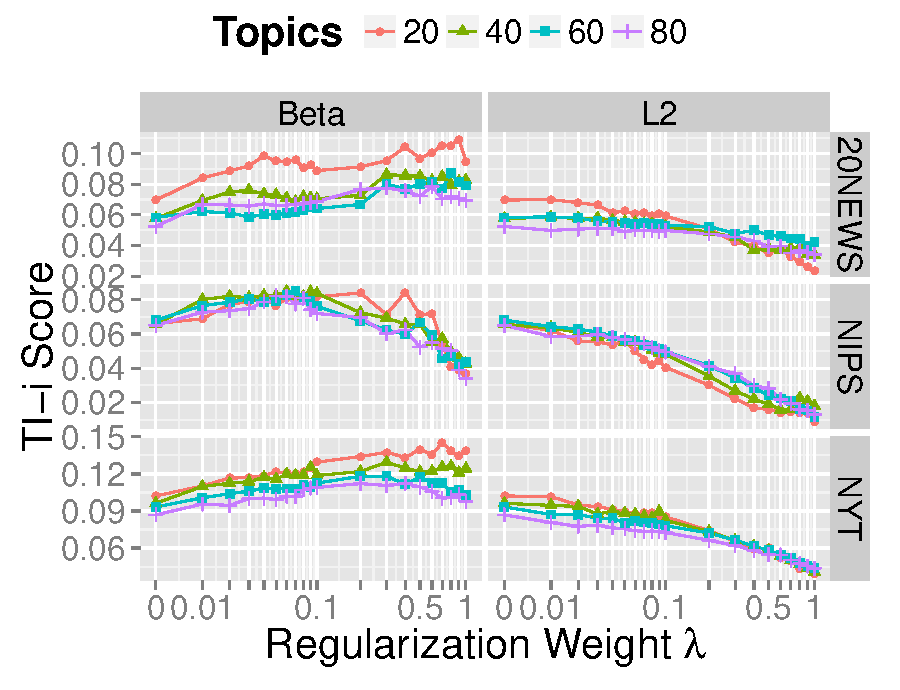
\includegraphics[width=0.48\linewidth]{2014_acl_reganchor/figures/TI_TI.pdf}}
\caption{Selection of $\lambda$ based on \abr{hl} and \abr{ti}
  scores on the development set. The value of $\lambda =0$ is equivalent to the original {\bf
    anchor} algorithm; regularized versions find better solutions as
  the regularization weight $\lambda$ becomes non-zero.}
\label{fig:select-lambda}
\end{figure*}


\subsection{Grid Search for Parameters on Development Set}
\label{sec:parameter-search}

\paragraph{Anchor Threshold}

A good anchor word must have a unique, specific context but also
explain other words well.  A word that appears only once will have a
very specific cooccurence pattern but will explain other words'
coocurrence poorly because the observations are so
sparse.  As discussed in Section~\ref{sec:anchor}, the {\bf anchor}
method uses document frequency $M$ as a threshold to only consider
words with robust counts.

Because all regularizations benefit equally from higher-quality anchor
words, we use cross-validation to select the document frequency cutoff
$M$ using the unregularized {\bf anchor} algorithm.
Figure~\ref{fig:anchor-select} shows the performance of {\bf anchor}
with different $M$ on our three datasets with 20 topics for our two
measures \abr{hl} and \abr{ti}-i.

\paragraph{Regularization Weight}

Once we select a cutoff $M$ for each combination of dataset,
number of topics $K$ and a evaluation measure, we select a regularization weight
$\lambda$ on the development set.  Figure~\ref{fig:select-lambda}
shows that {\bf beta} regularization framework improves topic
interpretability \abr{ti}-i on all datasets and improved the held-out
likelihood \abr{hl} on \abr{20news}.  The $L_2$ regularization also
improves held-out likelihood \abr{hl}
 for the \abr{20news} corpus (Figure~\ref{fig:select-lambda}).

In the interests of space, we do not show the figures for selecting $M$
 and $\lambda$ using \abr{ti}-e, which is similar to \abr{ti}-i: {\bf
   anchor-beta} improves \abr{ti}-e score on all datasets, {\bf
   anchor-$L_2$} improves \abr{ti}-e on \abr{20news} and \abr{nips}
 with 20 topics and \abr{nyt} with 40 topics.

\subsection{Evaluating Regularization}

With document frequency $M$ and regularization weight $\lambda$
selected from the development set, we compare the performance of those
models on the test set.  We also compare with standard implementations
of Latent Dirichlet Allocation: Blei's \abr{ldac} ({\bf variational}) and
Mallet ({\bf mcmc}).  We run 100 iterations for \abr{ldac} and 5000
iterations for Mallet.

Each result is averaged over three random runs and appears in
Figure~\ref{fig:results}.  The highly-tuned, widely-used implementations
uniformly have better held-out likelihood than {\bf anchor}-based methods, but
the much faster {\bf anchor} methods are often comparable.  Within {\bf
  anchor}-based methods, $L_2$-regularization offers comparable held-out
likelihood as unregularized {\bf anchor}, while {\bf anchor-beta} often has
better interpretability.  Because of the mismatch between the specialized
vocabulary of \abr{nips} and the general-purpose language of Wikipedia,
\abr{ti}-e has a high variance.

\begin{figure*}[t]
\centering
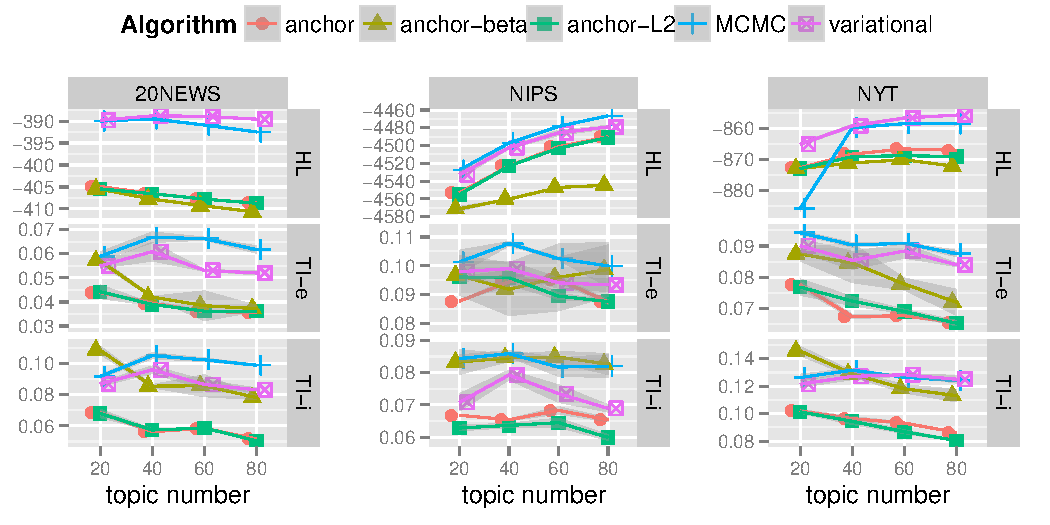
\includegraphics[width=\linewidth]{2014_acl_reganchor/figures/results_option3}
\caption{Comparing {\bf anchor-beta} and {\bf anchor-$L_2$} against
  the original {\bf anchor} and the traditional {\bf variational} and
  {\bf MCMC} on \abr{hl} score and \abr{ti} score.  {\bf variational}
  and {\bf mcmc} provide the best held-out generalization.  {\bf
    anchor-beta} sometimes gives the best \abr{ti} score and is
  consistently better than {\bf anchor}.  The specialized vocabulary
  of \abr{nips} causes high variance for the extrinsic
  interpretability evaluation (\abr{ti}-e).}
\label{fig:results}
\end{figure*}

\begin{table*}[t!]
\begin{small}
   \begin{center}

\begin{tabular}{|p{1cm}|c|p{8cm}|} \hline
Topic & Shared Words & Original (Top, green) vs. Informed $L_2$ (Bottom, orange) \\ \hline
\multirow{2}{*}{soviet}	&	\multirow{2}{5cm}{american make president {\bf soviet} union {\bf war} years } &	\cellcolor{green!30}gorbachev moscow russian force economic world europe political communist lead reform germany country \\&	&	\cellcolor{orange!30}{\bf military} state {\bf service} washington \red{bush} {\bf army} unite {\bf chief} {\bf troops} {\bf officer} \red{nuclear} time week \\ \hline
\multirow{2}{*}{district}	&	\multirow{2}{5cm}{{\bf assembly} board city {\bf county} {\bf district} {\bf member} state york } &	\cellcolor{green!30}representative manhattan brooklyn queens election bronx council island local incumbent housing municipal \\&	&	\cellcolor{orange!30}{\bf people} {\bf party} {\bf group} {\bf social} \red{republican} year make years {\bf friend} \red{vote} {\bf compromise} million \\ \hline
\multirow{2}{*}{peace}	&	\multirow{2}{5cm}{american force government israel {\bf peace} political president state unite washington } &	\cellcolor{green!30}war military country minister leaders nation world palestinian israeli election \\&	&	\cellcolor{orange!30}{\bf offer} {\bf justice} {\bf aid} {\bf deserve} make \red{bush} years {\bf fair} \red{clinton} {\bf hand} \\ \hline
\end{tabular}
\begin{tabular}{|p{1cm}|c|p{7cm}|} \hline
\multirow{2}{*}{arms}	&	\multirow{2}{6cm}{{\bf arms} bush congress force iraq make north nuclear president state washington weapon } &	\cellcolor{green!30}administration treaty missile defense war military korea reagan \\&	&	\cellcolor{orange!30}{\bf agree} {\bf agreement} american {\bf accept} unite {\bf share} \red{clinton} years \\ \hline
\multirow{2}{*}{trade}	&	\multirow{2}{6cm}{{\bf administration} america american country {\bf economic} government make president state {\bf trade} unite washington } &	\cellcolor{green!30}world market japan foreign china policy price political \\&	&	\cellcolor{orange!30}{\bf business} {\bf economy} \red{congress} year years \red{clinton} \red{bush} {\bf buy} \\ \hline
\end{tabular}

   \end{center}
\end{small}
\caption{Examples of topic comparison between {\bf anchor} and informed {\bf
    anchor-$L_2$}. A topic is labeled with the anchor word for that topic. The
  {\bf bold} words are the informed prior from \abr{liwc}. With an informed
  prior, relevant words appear in the top words of a topic; this also draws
  in other related terms (red). }
\label{tab:compare-informed}
\end{table*}

\subsection{Informed Regularization}
\label{sec:informed}

A frequent use of priors is to add information to a model.  This is not possible
with the existing {\bf anchor} method.  An informed prior for topic models seeds
a topic with words that describe a topic of interest.  In a topic model, these
seeds will serve as a ``magnet'', attracting similar words to the
topic~\cite{zhai-12}.

We can achieve a similar goal with {\bf anchor-$L_2$}.  Instead of
encouraging anchor coefficients to be zero in
Equation~\ref{eq:anchorl2}, we can instead encourage word
probabilities to close to an arbitrary mean $\mu_{i,k}$.  This vector
can reflect expert knowledge.

One example of a source of expert knowledge is Linguistic Inquiry and Word
Count~\cite[\abr{liwc}]{pennebaker-99}, a dictionary of keywords related to
sixty-eight psychological concepts such as \underline{positive emotions},
\underline{negative emotions}, and \underline{death}.  For example, it
associates ``excessive, estate, money, cheap, expensive, living, profit, live,
rich, income, poor, etc." for the concept \underline{materialism}.

We associate each anchor word with its closest \abr{liwc} category based on
the cooccurrence matrix $\bm{Q}$. This is computed by greedily finding the
anchor word that has the highest cooccurrence score for any \abr{liwc} category:
we define the score of a category to anchor word $w_{s_k}$ as $\sum_i Q_{s_k, i}$,
where $i$ ranges over words in this category; we compute the scores of all categories to
all anchor words; then we find the highest score and assign the category to that anchor
word; we greedily repeat this process until all anchor words have a category.

Given these associations, we create a goal mean $\mu_{i,k}$.  If there
are $L_i$ anchor words associated with \abr{liwc} word $i$, $\mu_{i, k}
= \frac{1}{L_i}$ if this keyword $i$ is associated with anchor word
$w_{s_k}$ and zero otherwise.

We apply {\bf anchor-$L_2$} with informed priors on \abr{nyt}
with twenty topics and compared the topics against the
original topics from {\bf anchor}.  Table~\ref{tab:compare-informed}
shows that the topic with anchor word ``soviet'', when combined with
\abr{liwc}, draws in the new words
``bush'' and ``nuclear''; reflecting the threats of force during the
cold war.  For the topic with topic word ``arms'', when associated
with the \abr{liwc} category \underline{} with the terms ``agree'' and
``agreement'', draws in ``clinton'', who represented a more
conciliatory foreign policy compared to his republican predecessors.

\section{Discussion}
\label{sec:disc}

Having shown that regularization can improve the {\bf anchor} topic
modeling algorithm, in this section we discuss \emph{why} these regularizations can
improve the model and the implications for practitioners.

\paragraph{Efficiency}

Efficiency is a function of the number of iterations and the cost of
each iteration.  Both {\bf anchor} and {\bf anchor-$L_2$} require a
single iteration, although the latter's iteration is slightly more
expensive.  For {\bf beta}, as described in Section~\ref{sec:beta}, we
update anchor coefficients $C$ row by row, and then repeat the process
over several iterations until it converges.  However, it often
converges within ten iterations (Figure~\ref{fig:convergence}) on all
three datasets: this requires much fewer iterations than \abr{mcmc} or variational
inference, and the iterations are less expensive.  In addition, since
we optimize each row $C_{i,\cdot}$ independently, the algorithm can be
easily parallelized.

\begin{figure}[t!]
\centering
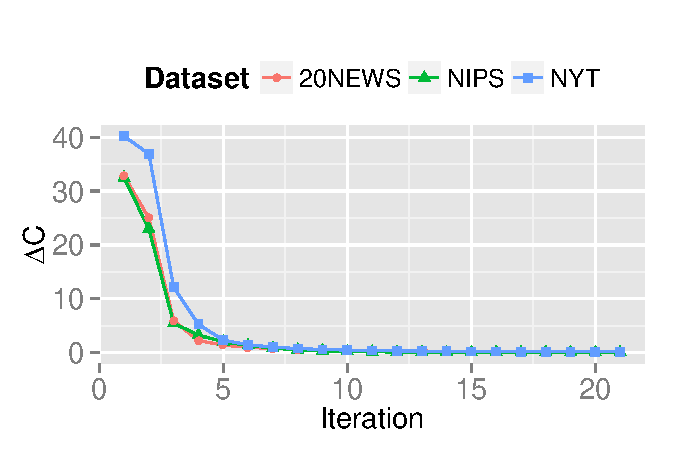
\includegraphics[width=\linewidth]{2014_acl_reganchor/figures/Convergence_C.pdf}
\caption{Convergence of anchor coefficient $C$ for {\bf anchor-beta}.
$\Delta C$ is the difference of current $C$ from the $C$ at the previous iteration.
$C$ is converged within ten iterations for all three datasets.}
\label{fig:convergence}
\end{figure}

\paragraph{Sensitivity to Document Frequency}

While the original {\bf anchor} is sensitive to the document frequency $M$
(Figure~\ref{fig:anchor-select}), adding regularization makes this less
critical.  Both {\bf anchor-$L_2$} and {\bf anchor-beta} are less sensitive to
$M$ than {\bf anchor}.

To highlight this, we compare the topics of {\bf anchor} and {\bf anchor-beta}
when $M=100$.  As Table~\ref{tab:sensitive-m} shows, the words
``article'', ``write'', ``don'' and ``doe'' appear in most of {\bf
  anchor}'s topics. While {\bf anchor-$L_2$} also has some bad
topics, it still can find reasonable topics, demonstrating {\bf
  anchor-beta}'s greater robustness to suboptimal $M$.



\begin{table*}[t!]
\begin{small}
   \begin{center}
\begin{tabular}{|c|p{6cm}|p{6cm}|} \hline
{\bf Topic} & {\bf anchor} & {\bf anchor-beta} \\ \hline
frequently & \green{article} \red{write} \blue{don} \purple{doe} make time people good file question & \green{article} \red{write} \blue{don} \purple{doe} make people time good email file \\ \hline
debate & \red{write} \green{article} people make \blue{don} \purple{doe} god key government time & people make god \green{article} \red{write} \blue{don} \purple{doe} key point government \\ \hline
wings & game team \red{write} wings \green{article} win red play hockey year & game team wings win red hockey play season player fan \\ \hline
stats & player team \red{write} game \green{article} stats year good play \purple{doe} & stats player season league baseball fan team individual playoff nhl \\ \hline
compile & program file \red{write} email \purple{doe} windows call problem run \blue{don} & compile program code file ftp advance package error windows sun \\ \hline
\end{tabular}

   \end{center}
\end{small}
\caption{Topics from {\bf anchor} and {\bf anchor-beta} with $M=100$ on \abr{20news} with 20 topics.
  Each topic is identified with its associated anchor word.
  When $M=100$, the topics of {\bf anchor} suffer: the four colored words appear in almost every topic.
  {\bf anchor-beta}, in contrast, is less sensitive to suboptimal $M$. }
\label{tab:sensitive-m}
\end{table*}


\paragraph{$L_2$ (Sometimes) Improves Generalization}

As Figure~\ref{fig:select-lambda} shows, {\bf anchor-$L_2$} sometimes
improves held-out development likelihood for the smaller
\abr{20news} corpus.  However, the $\lambda$ selected on development data does
not always improve test set performance.  This, in Figure~\ref{fig:results},
{\bf anchor-beta} closely tracks {\bf anchor}.  Thus, $L_2$ regularization does
not hurt generalization while imparting expressiveness and
robustness to parameter settings.

\paragraph{Beta Improves Interpretability}

Figure~\ref{fig:results} shows that {\bf anchor-beta} improves topic
interpretability (\abr{ti}) compared to unregularized anchor methods.
In this section, we try to understand why.

We first compare the topics from the original {\bf anchor} against {\bf
  anchor-beta} to analyze the topics qualitatively.
Table~\ref{tab:compare-beta} shows that {\bf beta} regularization promotes rarer
words within a topic and demotes common words.  For example, in the topic about
hockey with the anchor word \underline{game}, ``run'' and ``good''---ambiguous,
polysemous words---in the unregularized topic are replaced by ``playoff'' and
``trade'' in the regularized topic.  These words are less ambiguous and more
likely to make sense to a consumer of topic models.

Figure~\ref{fig:density-plot} shows why this happens.  Compared to the
unregularized topics from {\bf anchor}, the beta regularized topic steals from the rich and
creates a more uniform distribution.  Thus, highly frequent words do not as
easily climb to the top of the distribution, and the topics reflect topical,
relevant words rather than globally frequent terms.

\begin{figure*}[t!]
\centering
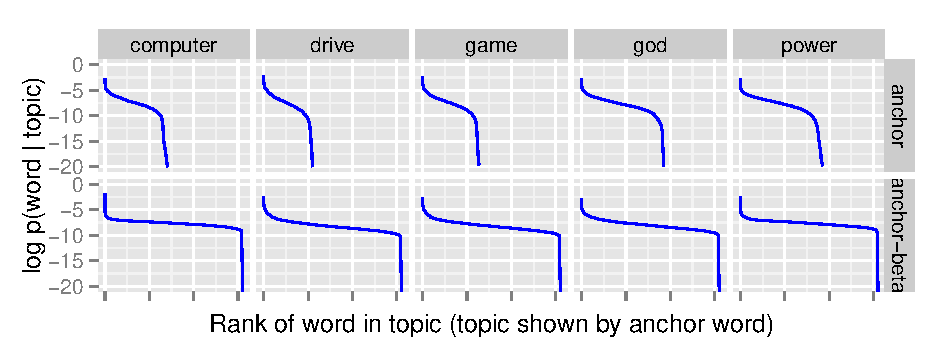
\includegraphics[width=0.9\linewidth]{2014_acl_reganchor/figures/density}
\caption{How beta regularization influences the topic distribution.  Each topic
  is identified with its associated anchor word.  Compared to the unregularized
  {\bf anchor} method, {\bf anchor-beta} steals
  probability mass from the ``rich'' and prefers a smoother distribution of
  probability mass.  These words often tend to be unimportant, polysemous words
  common across topics.
}
\label{fig:density-plot}
\end{figure*}

\begin{table*}[t!]
\begin{small}
   \begin{center}
       \begin{tabular}{|p{1.2cm}|c|p{8cm}|} \hline
           Topic & Shared Words & {\bf anchor} (Top, green) vs. {\bf anchor-beta} (Bottom, orange) \\ \hline
\multirow{2}{*}{computer}	&	\multirow{2}{4cm}{computer means science screen}	&	\cellcolor{green!30}system phone university problem doe work windows internet software chip mac set fax technology information data\\
&	&	\cellcolor{orange!30}quote mhz pro processor ship remote print devices complex cpu electrical transfer ray engineering serial reduce\\ \hline

\multirow{2}{*}{power}	&	\multirow{2}{4cm}{power play period supply ground light battery engine}	&	\cellcolor{green!30}car good make high problem work back turn control current small time\\
&	&	\cellcolor{orange!30}circuit oil wire unit water heat hot ranger input total joe plug\\ \hline
\end{tabular}

\begin{tabular}{|p{1.2cm}|c|p{5cm}|} \hline
\multirow{2}{*}{god}	&	\multirow{2}{7cm}{god jesus christian bible faith church life christ belief religion hell word lord truth love}	&	\cellcolor{green!30}people make things true doe\\
&	&	\cellcolor{orange!30}sin christianity atheist peace heaven\\ \hline

\multirow{2}{*}{game}	&	\multirow{2}{7cm}{game team player play win fan hockey season baseball red wings score division league goal leaf cup toronto}	&	\cellcolor{green!30}run good\\
&	&	\cellcolor{orange!30}playoff trade\\ \hline

\multirow{2}{*}{drive}	&	\multirow{2}{7cm}{drive disk hard scsi controller card floppy ide mac bus speed monitor switch apple cable internal port meg}	&	\cellcolor{green!30}problem work\\
&	&	\cellcolor{orange!30}ram pin\\ \hline
\end{tabular}

  \end{center}
\end{small}
\caption{Comparing topics---labeled by their anchor word---from {\bf
    anchor} and {\bf anchor-beta}. With beta regularization, relevant
  words are promoted, while more general words are suppressed,
  improving topic coherence.}
\label{tab:compare-beta}
\end{table*}
\section{Conclusion}
\label{sec:conclusion}

A topic model is a popular tool for quickly getting the gist of large
corpora.  However, running such an analysis on these large corpora
entail a substantial computational cost.  While techniques such as
{\bf anchor} algorithms offer faster solutions, it comes at the cost
of the expressive priors common in Bayesian formulations.

This paper introduces two different regularizations that offer users more
interpretable models and the ability to inject prior knowledge without
sacrificing the speed and generalizability of the underlying approach.  However,
one sacrifice that this approach does make is the beautiful theoretical
guarantees of previous work.  An important piece of future work is a theoretical
understanding of generalizability in extensible, regularized models.

Incorporating other regularizations could further improve performance
or unlock new applications.  Our regularizations do not explicitly
encourage sparsity; applying other regularizations such as $L_1$ could
encourage true sparsity~\cite{Tibshirani-1994}, and structured
priors~\cite{andrzejewski-09} could efficiently incorporate
constraints on topic models.

These regularizations could improve spectral
algorithms for latent variables models, improving the performance for
other \abr{nlp} tasks such as latent variable
\abr{pcfg}s~\cite{cohen-13b} and \abr{hmm}s~\cite{anandkumar-12:hmm},
combining the flexibility and robustness offered by priors with the
speed and accuracy of new, scalable algorithms.


\section*{Acknowledgments}

We would like to thank the anonymous reviewers, Hal Daum\'e III, Ke Wu,
and Ke Zhai for their helpful comments.  This work was supported by
\abr{nsf} Grant IIS-1320538.  Boyd-Graber is also supported by
\abr{nsf} Grant CCF-1018625.  Any opinions, findings, conclusions, or
recommendations expressed here are those of the authors and do not
necessarily reflect the view of the sponsor.

\newpage

%\bibliographystyle{style/icml2013}
\bibliographystyle{style/acl2014}
%\bibliographystyle{apalike}
%\footnotesize
\bibliography{bib/journal-full,bib/thang,bib/jbg,bib/ynhu}

\end{document}
